\subsection{Implementation}
\label{sec:allocator}

We implement \Mesh as a drop-in replacement memory allocator that
implements meshing for single or multi-threaded applications written
in C/C++. Its current implementation work for 64-bit Linux and Mac OS
X binaries. \Mesh can be explicitly linked against by passing
\texttt{-lmesh} to the linker at compile time, or loaded dynamically
by setting the \texttt{LD\_PRELOAD} (Linux) or
\texttt{DYLD\_INSERT\_LIBRARIES} (Mac OS X) environment variables to
point to the \Mesh{} library. When loaded, \Mesh interposes on
standard libc functions to replace all memory allocation functions.

\begin{comment}
\begin{figure}
  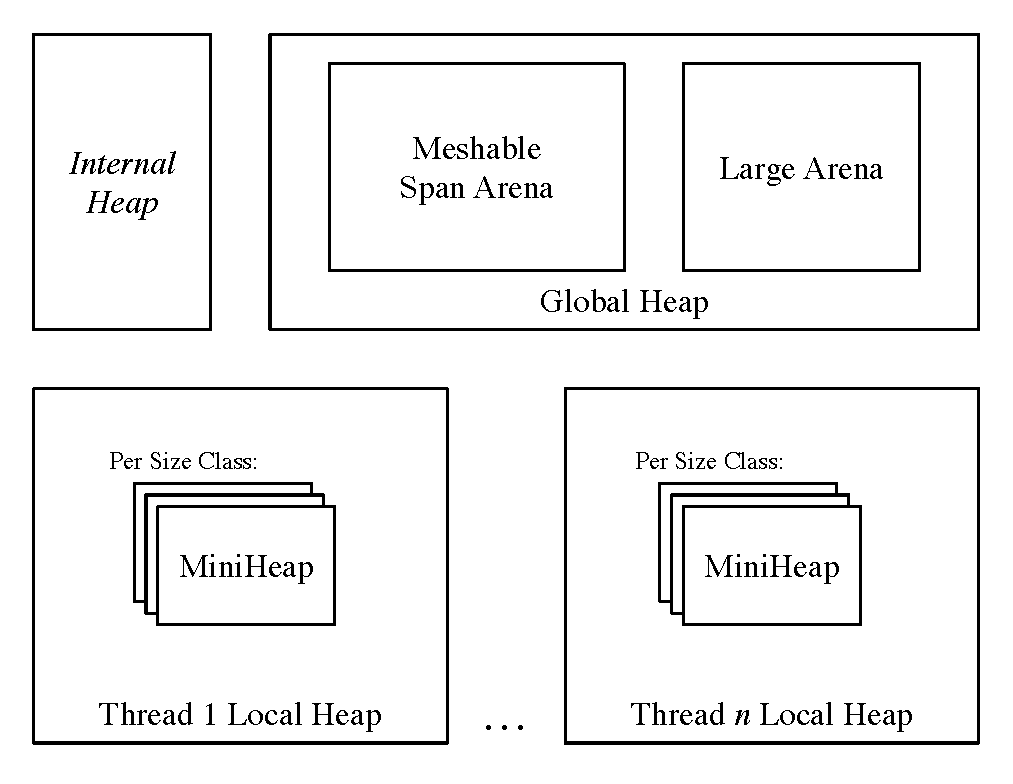
\includegraphics[width=.5\textwidth]{figures/global_heap}
  \caption{\textbf{Heap organization.} \Mesh's internal allocator
    manages memory for \Mesh-internal dynamic data structures.
    The global heap manages both large objects and the meshable arena that spans are allocated from.  Each thread has a
    local heap which satisfies small allocations from MiniHeaps (one
    per size class).}
  \label{fig:global-heap}
\end{figure}
\end{comment}

\Mesh combines traditional allocation strategies with meshing to
minimize heap usage.  Like most modern memory
allocators~\cite{Novark:2010:DSH:1866307.1866371,1134000,379232,evans2006scalable,ghemawattcmalloc},
\Mesh is a segregated-fit allocator. \Mesh{} employs fine-grained size
classes to reduce internal fragmentation due to rounding up to the
nearest size class. \Mesh{} uses the same size classes as those
used by jemalloc for objects 1024 bytes and
smaller~\cite{evans2006scalable}, and power-of-two size classes for
objects between 1024 and 16K.  Allocations are fulfilled from the
smallest size class they fit in (e.g., objects of size 33--48 bytes
are served from the 48-byte size class); objects larger than 16K are
individually fulfilled from the global arena.  Small objects are
allocated out of \textit{spans} (\S\ref{sec:meshing}), which are
multiples of the page size and contain between 8 and 256 objects of a
fixed size.  Having at least eight objects per span helps
amortize the cost of reserving memory from the global manager for
the current thread's allocator.

Objects of 4KB and larger are always page-aligned and span at least one
entire page. \Mesh does not consider these objects for meshing;
instead, the pages are directly freed to the OS.

\Mesh's heap organization consists of four main components.
\emph{MiniHeaps} track occupancy and other metadata for spans.
%(\S\ref{sec:miniheaps}).  
\textit{Shuffle vectors} enable efficient,
random allocation out of a MiniHeap. %(\S\ref{sec:shuffle-freelists}).
\textit{Thread local heaps} satisfy small-object allocation requests
without the need for locks or atomic operations in the common case.
%(\S\ref{sec:thread-local-heaps}). 
Finally, the \textit{global heap}
(\S\ref{sec:global-heap}) manages runtime state shared by all threads,
large object allocation, and coordinates meshing operations.
%(\S\ref{sec:meshing-implementation}).
We omit detailing discussion of these components of \Mesh in this document.


\iffalse

\subsection{MiniHeaps}
\label{sec:miniheaps}

MiniHeaps manage allocated physical spans of memory and are either
\emph{attached} or \emph{detached}.  An attached MiniHeap is owned by
a specific thread-local heap, while a detached MiniHeap is only
referenced through the global heap.  New small objects are
\textit{only} allocated out of attached MiniHeaps.

Each MiniHeap contains metadata that comprises span length, object
size, allocation bitmap, and the start addresses of any virtual spans
meshed to a unique physical span.  The number of objects that can be
allocated from a MiniHeap bitmap is \textit{objectCount = spanSize /
  objSize}.  The allocation bitmap is initialized to
\textit{objectCount} zero bits.

When a MiniHeap is attached to a
thread-local \emph{shuffle vector} (\S\ref{sec:shuffle-freelists}),
each offset that is unset in the MiniHeap's bitmap is added to the
shuffle vector, with that bit now atomically set to one in the bitmap.
This approach is designed to allow multiple threads to free objects
which keeping most memory allocation operations local in the common
case.

When an object is freed and the free is non-local
(\S\ref{sec:deallocation-algorithm}), the bit is reset.  When a new
MiniHeap is allocated, there is only one virtual span that points to
the physical memory it manages. After meshing, there may be multiple
virtual spans pointing to the MiniHeap's physical memory.


\begin{figure}[!t]
  \centering
  \subfloat[A shuffle vector for a span of size 8, where no objects have
      yet been allocated.]{
      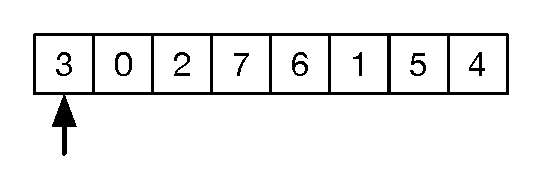
\includegraphics[width=.4\textwidth]{Chapters/mesh/figures/shuffle-freelist_a}
  }
  \vspace{-0em}
  \subfloat[The shuffle vector after the first object has been allocated.]{
      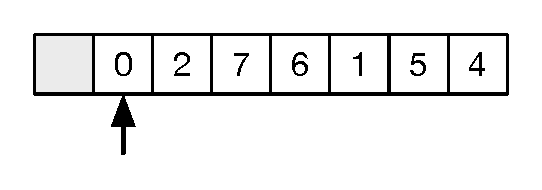
\includegraphics[width=.4\textwidth]{Chapters/mesh/figures/shuffle-freelist_b}
  }
  \vspace{-0em}
  \subfloat[On \texttt{free}, the object's offset is pushed onto the
      front of the vector, the allocation index is updated, and the
      offset is swapped with a randomly chosen offset.]{
      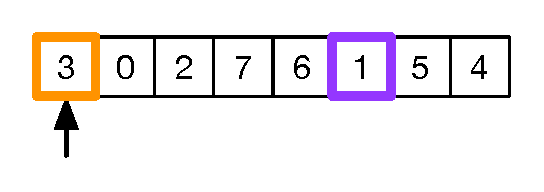
\includegraphics[width=.4\textwidth]{Chapters/mesh/figures/shuffle-freelist_c}
  }
  \vspace{-0em}
  \subfloat[Finally, after the swap, new allocations proceed in a
      bump-pointer like fashion.]{
    \centering
    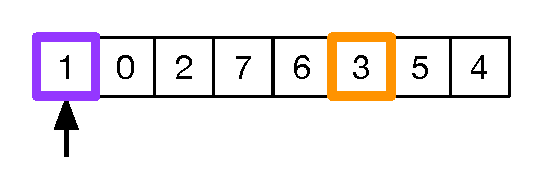
\includegraphics[width=.4\textwidth]{Chapters/mesh/figures/shuffle-freelist_d}
  }
  \vspace{0.5em}
  \caption{\textbf{Shuffle vectors} compactly enable fast random allocation.
    Indices (one byte each) are maintained in random order; allocation is
    popping, and deallocation is pushing plus a random swap (\S\ref{sec:shuffle-freelists}).}
    % When an object is freed and the MiniHeap     it was allocated from is still attached to the local thread,    its
  \label{fig:shuffle-freelists}
\end{figure}


%% TODO: restore locality section if and when we have locality results
\begin{comment}
\subsubsection{Locality}

At first blush, it may appear that \Mesh's use of randomization would
degrade locality and thus degrade performance. Like DieHard (but unlike
many other allocators), \Mesh does not seek to allocate consecutive
objects nearby. However, we expect this approach to have minimal
impact on locality in many cases. First, the increasing size of cache
lines means that inter-object locality is not a concern for most
objects. Modern 64-bit Intel processors have 64-byte cache lines, and
ARM devices have 32 or 64-byte cache lines, meaning that object
locality has little impact on L1 cache locality for objects of that
size or larger. We also expect TLB pressure to be unaffected compared
to other segregated-fit allocators with the same choice of size
classes; \Mesh allocates randomly \emph{within} spans. % \textbf{XXX forward ref to evaluation; we want to say primary cost is allocation mechanism, not locality effects.}
\end{comment}

\subsection{Shuffle Vectors}
\label{sec:shuffle-freelists}

Shuffle vectors are a novel data structure that lets \Mesh
perform randomized allocation out of a MiniHeap efficiently and
with low space overhead.

Previous memory allocators that have employed randomization (for
security or reliability) perform randomized allocation by random
probing into
bitmaps~\cite{1134000,Novark:2010:DSH:1866307.1866371}. In these
allocators, a memory allocation request chooses a random number in the
range $[0,\text{\textit{objectCount}}-1]$. If the associated bit is
zero in the bitmap, the allocator sets it to one and returns the
address of the corresponding offset. If the offset is already one,
meaning that the object is in use, a new random number is chosen and
the process repeated. Random probing allocates objects in $O(1)$
\emph{expected} time but requires overprovisioning memory by a
constant factor (e.g., $2\times$ more memory must be allocated than
needed). This overprovisioning is at odds with our goal of
\emph{reducing} space overhead.

Shuffle vectors solve this problem, combining low space overhead with
worst-case $O(1)$ running time for \texttt{malloc} and
\texttt{free}. Each comprises a fixed-size array consisting of all the
offsets from a span that are \textit{not} already allocated, and an
allocation index representing the head. Each vector is initially
randomized with the Knuth-Fischer-Yates
shuffle~\cite{knuth:1981:semi}, and its allocation index is set to
0. Allocation proceeds by selecting the next available number in the
vector, ``bumping'' the allocation index and returning the
corresponding address. Deallocation works by placing the freed object
at the front of the vector and performing one iteration of the shuffle
algorithm; this operation preserves randomization of the
vector. Figure~\ref{fig:shuffle-freelists} illustrates this process,
while Figure~\ref{fig:malloc} has pseudocode listings for
initialization, allocation, and deallocation.

%\vspace{-1.2em}
%\begin{align*}
 % \text{\textit{ptr}} = \text{\textit{spanStart + off*objSize}}
%\end{align*}

%This freelist is initialized with all of the available offsets $[0
%  .. $ objectCount $]$ and then sorted

%When an object is freed and the owning MiniHeap is still in use, a
%single iteration of the shuffle is performed to re-add the newly freed
%offset back to the list of available offsets.

Shuffle vectors impose far less space overhead than random
probing. First, with a maximum of 256 objects in a span, each offset
in the vector can be represented as an unsigned character (a single
byte). Second, because \Mesh needs only one shuffle vector per
attached MiniHeap, the amount of memory required for vectors is
$256c$, where $c$ is the number of size classes (24 in the current
implementation): roughly 2.8K per thread.  Finally, shuffle vectors
are only ever accessed from a single thread, and so do not require
locks or atomic operations.  While bitmaps must be operated on
atomically (frees may originate at any time from other threads),
shuffle vectors are only accessed from a single thread and do not
require synchronization or cache-line flushes.

\subsection{Thread Local Heaps}
\label{sec:thread-local-heaps}

All malloc and free requests from an application start at the thread's
local heap. Thread local heaps have shuffle vectors for each size
class, a reference to the global heap, and their own thread-local
random number generator.

Allocation requests are handled differently depending on the size of
the allocation.  If an allocation request is larger than 16K, it is
forwarded to the global heap for fulfillment
(\S\ref{sec:global-heap}).  Allocation requests 16K and smaller are
small object allocations and are handled directly by the shuffle
vector for the size class corresponding to the allocation request, as
in Figure~\ref{fig:malloc}a.  If the shuffle vector is empty, it is
refilled by requesting an appropriately sized MiniHeap from the global
heap.  This MiniHeap is a partially-full MiniHeap if one exists, or
represents a freshly-allocated span if no partially full ones are
available for reuse.  Frees, as in Figure~\ref{fig:malloc}d, first
check if the object is from an attached MiniHeap.  If so, it is
handled by the appropriate shuffle vector, otherwise it is passed to
the global heap to handle.

\subsection{Global Heap}
\label{sec:global-heap}

The global heap allocates MiniHeaps for thread-local heaps, handles
all large object allocations, performs non-local frees for both small
and large objects, and coordinates meshing.

\subsubsection{The Meshable Arena}
\label{sec:meshable-arena}

The global heap allocates meshable spans and large objects from a
single, global meshable arena. This arena contains two sets of bins
for same-length spans --- one set is for demand zero-ed spans (freshly
\texttt{mmap}ped), and the other for used spans --- and a mapping of
page offsets from the start of the arena to their owning MiniHeap
pointers.  Used pages are not immediately returned to the OS as they
are likely to be needed again soon, and reclamation is relatively
expensive. Only after 64MB of used pages have accumulated, or whenever
meshing is invoked, \Mesh{} returns pages to OS by calling
\texttt{fallocate} on the heap's file descriptor
(\S\ref{sec:page-table-updates}) with the
\texttt{FALLOC\_FL\_PUNCH\_HOLE} flag.

\begin{comment}
An allocation request for $k$ pages is fulfilled by searching through
the bins of free spans from index $k-1$ to $k_{\text{max}}$ for a free
span of at-least size $k$.  Bins smaller than $k_{\text{max}}$ only
contain spans of a single size, while $k_{\text{max}}$ contains spans
of length 256 or larger.  If no spans are available, the arena is
extended, the extension placed in $k_{\text{max}}$, and bins are
re-searched.  Once a resulting span has been found, if the span is
larger than the $k$ pages requested it is broken in two with the
remainder span placed back in an appropriate bin.  This scheme favors
dirty pages over clean pages to minimize the process's RSS.
\end{comment}

% TODO: mention how this is also how aligned allocations work

\begin{figure}[!t]
  \centering
  \subfloat{\lstinputlisting[language=C++, basicstyle=\footnotesize]{Chapters/mesh/all-code1}}
  \centering
  \subfloat{\lstinputlisting[language=C++, basicstyle=\footnotesize]{Chapters/mesh/all-code2}}
  %
void *MeshLocal::malloc(size_t sz) {
  
  int szClass;
  // forward to global heap if large
  if (!getSizeClass(sz, &szClass))
    return _global->malloc(sz);
  auto shufVec = _shufVecs[szClass];
  if (shufVec.isExhausted()) {
    shufVec.detachMiniheap();
    shufVec.attach(
      _global->allocMiniheap(szClass));}
  return shufVec.malloc();
}

void ShuffleVector::attach(MiniHeap *mh){
  _mh = mh;
  _off = maxCount();
  for (auto i = 0; i < maxCount(); i++){
    // true if atomically set (0 -> 1)
    if (bitmap.tryToSet(i)) {
      _list[_off--] = i;
    } }
  shuffle(_list[_off],
          _list[maxCount()]);
}


  %

void *ShuffleVector::malloc() {
  const auto off = _list[_off++];
  return _spanStart + off * _objSize;
}

void MeshLocal::free(void *ptr) {
  // check if in attached MiniHeap
  for (auto i=0; i<SizeClassCount; i++){
    const auto curr = _shufVecs[i];
    if (curr->contains(ptr)) {
      curr->free(ptr);
      return; } }
  _global->free(ptr); // general case
}

void ShuffleVector::free(void *ptr) {
  const auto freedOff = getOff(ptr);
  _list[--_off] = freedOff;
  // place newly freed address
  // randomly in the shuffle vector
  auto swapOff =
    _rng.inRange(_off, maxCount() - 1);
  swap(_list[_off], _list[swapOff]);
}


%  \input{./local-malloc.cc}
%  \input{./freelist-attach.cc}
%  \input{./miniheap-malloc.cc}
%  \input{./local-free.cc}
%  \input{./miniheap-free.cc}
  \caption{Pseudocode for \Mesh's core allocation and deallocation routines.}
  \label{fig:malloc}
\end{figure}



\subsubsection{MiniHeap Allocation}

Allocating a MiniHeap of size $k$ pages begins with requesting $k$
pages from the meshable arena.  The global allocator then allocates
and initializes a new MiniHeap instance from an internal allocator
that \Mesh uses for its own needs. This MiniHeap is kept live so long
as the number of allocated objects remains non-zero, and singleton
MiniHeaps are used to account for large object allocations.  Finally,
the global allocator updates the mapping of offsets to MiniHeaps for
each of the $k$ pages to point at the address of the new MiniHeap.

\subsubsection{Large Objects}

All large allocation requests (greater than 16K) are directly
handled by the global heap. Large allocation requests are rounded up
to the nearest multiple of the hardware page size (4K on x86\_64),
and a MiniHeap for 1 object of that size is requested, as detailed
above.  The start of the span tracked by that MiniHeap is returned to
the program as the result of the malloc call.

\subsubsection{Non-local Frees}

If \texttt{free} is called on a pointer that is not contained in an
attached MiniHeap for that thread, the free is handled by the global
heap.  Non-local frees occur when the thread that frees the object is
different from the thread that allocated it, or if there have been
sufficient allocations on the current thread that the original
MiniHeap was exhaused and a new MiniHeap for that size class was
attached.

Looking up the owning MiniHeap for a pointer is a constant time
operation. The pointer is checked to ensure it falls within the arena,
the arena start address is subtracted from it, and the result is
divided by the page size.  The resulting offset is then used to index
into a table of MiniHeap pointers. If the result is zero, the pointer
is invalid; otherwise, it points to a live MiniHeap.  This enables us
to catch certain application-level memory management errors, like
non-local double frees when a new object hasn't been allocated at the
same address.

Once the owning MiniHeap has been found, that MiniHeap's bitmap is
updated atomically in a compare-and-set loop.  If a free occurs for an
object where the owning MiniHeap is attached to a different thread,
the free atomically updates that MiniHeap's bitmap, but does not
update the other thread's corresponding shuffle vector.


\subsection{Meshing}
\label{sec:meshing-implementation}

\Mesh's implementation of meshing is guided by theoretical results
(described in detail in Section~\ref{sec:theory}) that enable it to
efficiently find a number of spans that can be meshed.

Meshing is rate limited by a configurable parameter, settable at
program startup and during runtime by the application through the
semi-standard \texttt{mallctl} API.  The default rate meshes at most
once every tenth of a second.  If the last meshing freed less than one
MB of heap space, the timer is not restarted until a subsequent
allocation is freed through the global heap.  This approach ensures that \Mesh
does not waste time searching for meshes when the application and heap
are in a steady state.

We implement the \sm algorithm from Section~\ref{sec:algorithms} in
C++ to find meshes.  Meshing proceeds one size class at a time.  Pairs
of mesh candidates found by \sm are recorded in a list, and after \sm
returns candidate pairs are meshed together \emph{en masse}.

Meshing spans together is a two step process. First, \Mesh{}
consolidates objects onto a single physical span. This consolidation
is straightforward: \Mesh{} copies objects from one span into the free
space of the other span, and updates MiniHeap metadata (like the
allocation bitmap).  Importantly, as \Mesh copies data at the physical
span layer, even though objects are moving in memory, no pointers or
data internal to moved objects or external references need to be
updated. Finally, \Mesh{} updates the process's virtual-to-physical mappings
to point all meshed virtual spans at the consolidated physical
span.

Physical memory reclaimed from meshing in one size class is able to be
used to satisfy future allocations in other size classes.

\subsubsection{Page Table Updates}
\label{sec:page-table-updates}

\Mesh updates the process's page tables via calls to \texttt{mmap}.
We exploit the fact that \texttt{mmap} lets the same offset in a file
(corresponding to a physical span) be mapped to multiple
addresses. \Mesh's arena, rather than being an anonymous mapping, as
in traditional \texttt{malloc} implementations, is instead a shared mapping
backed by a temporary file. This temporary file is obtained via the
\texttt{memfd\_create} system call and only exists in memory or on
swap.


\subsubsection{Concurrent Meshing}

Meshing takes place concurrently with the normal execution of other
program threads with \textit{no} stop-the-world phase required.  This
is similar to how concurrent relocation is implemented in low-latency
garbage collector algorithms like Pauseless and
C4~\cite{click:2005:pauseless, tene:2011:c4}, as described below.
\Mesh maintains two invariants throughout the meshing process: reads
of objects being relocated are always correct and available to
concurrently executing threads, and objects are never written to while
being relocated between physical spans.  The first invariant is maintained
through the atomic semantics of \texttt{mmap}, the second through a
write barrier.

\Mesh's write barrier is implemented with page protections and a
segfault trap handler.  Before relocating objects, \Mesh calls
\texttt{mprotect} to mark the virtual page where objects are being
copied from as read-only.  Concurrent reads succeed as normal.  If a
concurrent thread tries to write to an object being relocated, a
\Mesh-controlled segfault signal handler is invoked by a combination
of the hardware and operating system.  This handler waits on a lock
for the current meshing operation to complete, the last step of which
is remapping the source virtual span as read/write.  Once meshing is
done the handler checks if the address that triggered the segfault was
involved in a meshing operation; if so, the handler exits and the
instruction causing the write is re-executed by the CPU as normal
against the fully relocated object.


\subsubsection{Concurrent Allocation}

All thread-local allocation (on threads other than the one running
\sm) can proceed concurrently and independently with meshing, until
and unless a thread needs a fresh span to allocate from.  Allocation
only is performed from spans owned by a thread, and only spans owned
by the global manager are considered for meshing; spans have a single
owner.  The thread running \sm holds the global heap's lock while
meshing.  This lock also synchronizes transferring ownership of a span
from the global heap to a thread-local heap (or vice-versa).  If
another thread requires a new span to fulfill an allocation request,
the thread waits until the global manager finishes meshing and
releases the lock.

\subsection{Huge Pages}

Mesh's heap is not designed to be used in conjunction with transparent
huge pages, where the page table size used by the kernel and hardware
is 2MB rather than 4KB and the kernel runs a garbage collection-like
daemon to coalesce 4KB pages into 2MB pages.  Huge pages reduce TLB
pressure, but necessarily increase the granularity at which the kernel
manages physical memory on behalf of the process. This coarse
granularity is fundamentally at odds with Mesh's focus on minimizing
heap size.  Additionally, the \texttt{madvise} mechanism that Mesh and
other allocators like jemalloc use to return memory to the OS
interacts poorly with transparent huge pages on Linux (causing 2MB
pages to be split into 4KB pages), to the extent that major software
vendors and operators recommend disabling transparent huge pages
altogether~\cite{cloudera:thb,redis:thb,mongodb:thb,oracle:thb,nelson:thb}.
Applications that need to back datasets or data structures with huge
pages can still directly allocate (non-Mesh-managed) memory from Linux
using one of several interfaces~\cite{lwn:hp-interfaces}.

%% Mainstream CPUs have incorporated hierarchical TLBs for 4 KB pages,
%% reducing the performance impact of TLB
%% pressure~\cite{anandtech:nehelem-tlb,vtune:page-walk}.  Additionally,
%% with transparent huge pages on Linux, there is a high cost in finding
%% pages to physically relocate, in order to convert contiguous chunks of
%% memory from traditional to huge pages.  Many databases and server
%% workloads like redis~\cite{redis:thb}, MongoDB~\cite{mongodb:thb}, and
%% Oracle~\cite{oracle:thb} recommend disabling transparent huge pages.


\fi